% How to use foreach loop in LaTeX?
% http://latexdraw.com
% 12/12/2019, 20:43


\documentclass{standalone}

\usepackage{tikz}

\begin{document}

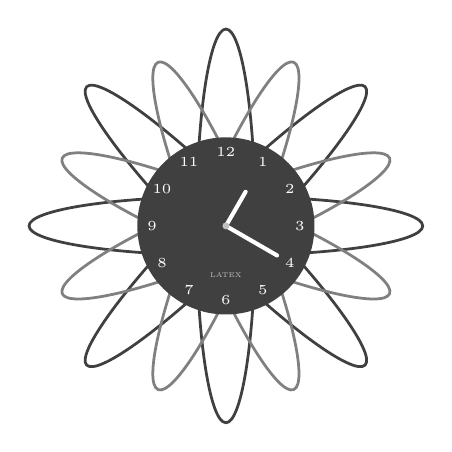
\begin{tikzpicture}[scale=1.25]
{\foreach \anglea in {0,45,...,135}
\draw[rotate=\anglea,line width =1pt, draw=black!75] (0,0) ellipse(2 and 0.3);}
\foreach \angleb in {22.5,67.5,...,180}
\draw[rotate=\angleb,line width =1pt, draw=gray] (0,0) ellipse(1.8 and 0.3);
\fill[black!75] (0,0) circle(0.9);
\draw[line width=1.5pt, white,cap=round] (0,0) -- (60:0.4);
\draw[line width=1.5pt, white,cap=round] (0,0) -- (-30:0.6);
\fill[lightgray] (0,0) circle(1pt);
\foreach \angle / \label in {0/3, 30/2, 60/1, 90/12, 120/11, 150/10, 180/9,     210/8, 240/7, 270/6, 300/5, 330/4}
  { \draw (\angle:0.75) node[text=white]{\tiny{\label}};  }
\node[scale=0.5, text=lightgray] at (-90:0.5) {\tiny LATEX};
\end{tikzpicture}

\end{document}
